\section{Rationale}
\label{multi-version:rationale}

% All the scenarios presented above describe software updates which, while trying
% to fix existing bugs or refactor the code, also introduced new bugs that caused
% the code to crash under certain conditions. Improving the reliability of such
% updates is the main goal of our proposed approach: running both the old and the
% new version in parallel after an update can enable applications to survive more
% errors, without giving up the new features introduced by the update.

% The bottom line for all the presented scenarios is that for significant amount
% of time, \ie about one year in case of \lighttpd and six months in case of
% \redis, users affected by buggy patches essentially had to decide between%
% \begin{inparaenum}[(1)]
% \item incorporating other security and bug fixes added to the code, but being
%   vulnerable to these crash bug, and
% \item giving up on these security and bug fixes and using an old version of
%   \lighttpd or \redis, which are not vulnerable to these newly introduced bugs.
% \end{inparaenum}
% Note that this is particularly true for the period between the time when the
% bug was introduced and the time it was diagnosed (\ie eleven months in case of
% \lighttpd, six months in case of \redis), since during this period most users
% would not know how to change the server's configuration to avoid the crash.

All the scenarios presented above describe software updates which, while trying
to fix existing bugs or refactor the code, also introduced new bugs that caused
the code to crash under certain conditions. The bottom line for all these
scenarios is that for significant amount of time, \ie about one year in the
case of \lighttpd, six months in the case of \redis, and one month in the case
\vim, users affected by buggy patches essentially had to decide between%
\begin{inparaenum}[(1)]
\item incorporating other security and bug fixes added to the code, but being
  vulnerable to these crash bugs, and
\item giving up on these security and bug fixes and using an old version of
  \lighttpd or \redis, which are not vulnerable to these newly introduced bugs.
\end{inparaenum}
Note that this is particularly true for the period between the time when the
bug was introduced and the time it was diagnosed (\ie eleven months in case of
\lighttpd, six months in case of \redis), since during this period most users
would not know how to change the server's configuration to avoid the crash.

\begin{figure}[t]
  \begin{subfigure}[b]{0.475\textwidth}
    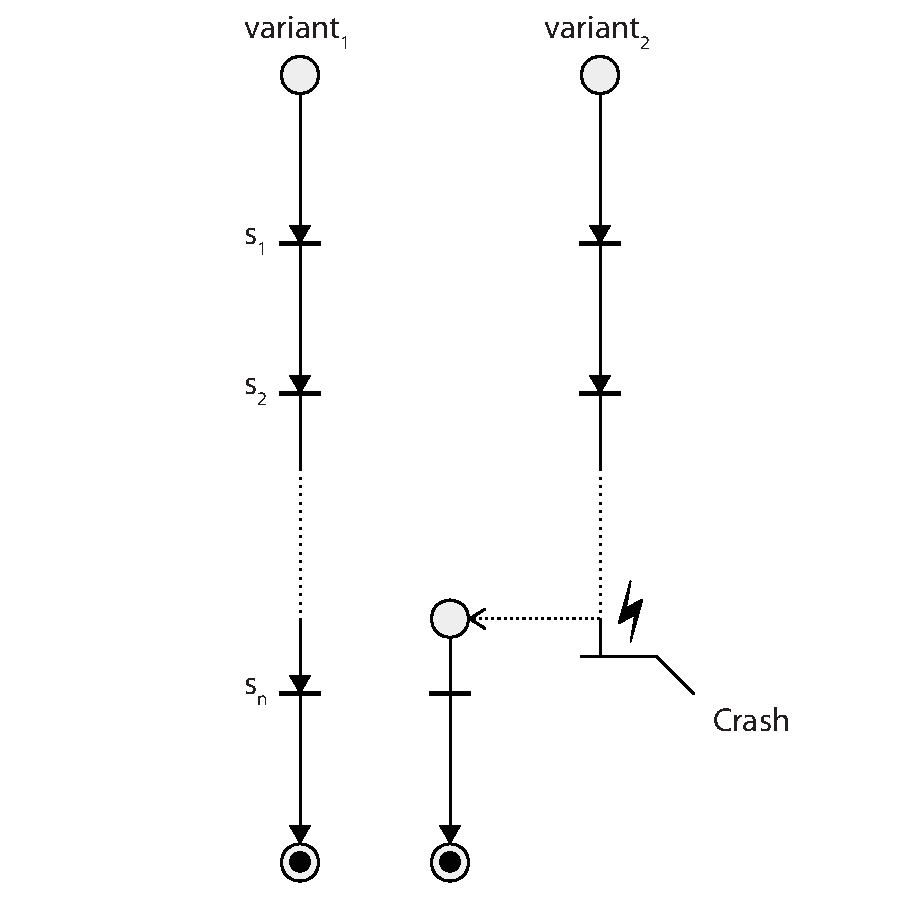
\includegraphics[width=\textwidth]{overview/figures/failrecovery}
    \caption{Failure recovery scheme.}
    \label{fig:failrecovery-scheme}
  \end{subfigure}
  \quad
  \begin{subfigure}[b]{0.475\textwidth}
    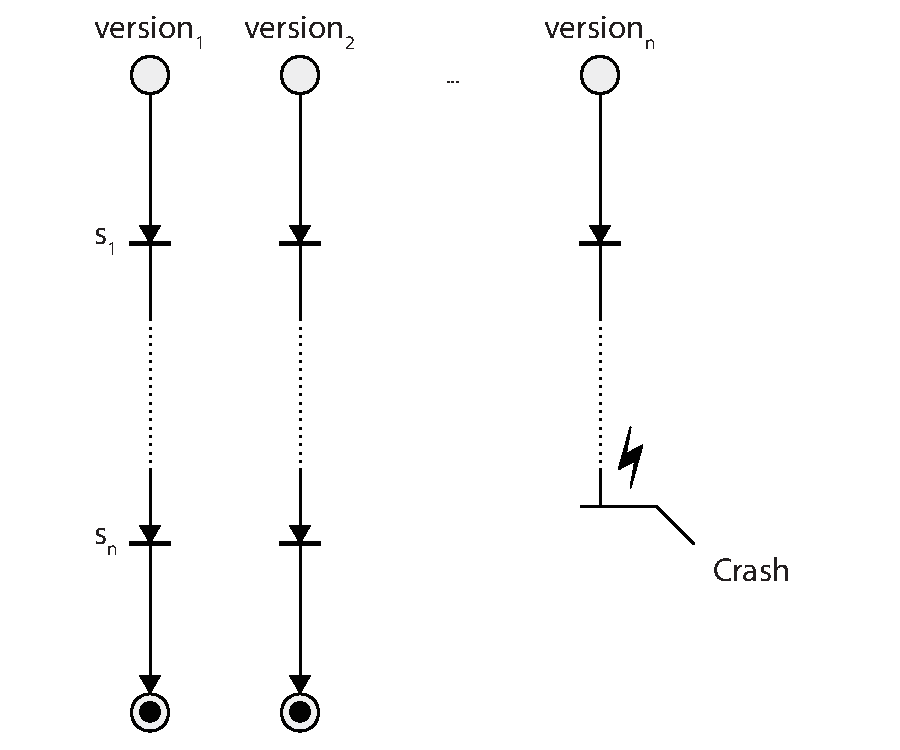
\includegraphics[width=\textwidth]{overview/figures/failover}
    \caption{Transparent failover scheme.}
    \label{fig:failover-scheme}
  \end{subfigure}
  \caption{Two schemes of multi-version execution presented in the thesis.}
  \label{fig:mvx-schemes}
\end{figure}

Our approach aims to provide users with a third choice: when a new version
becomes available, instead of replacing the old version, we will run both
versions in parallel; as new versions arrive, we continue to execute them in
parallel with the existing ones. Then, by selecting the output of the more
reliable version when their executions diverge, we can increase the overall
reliability of the software. There are multiple ways to implement this
approach. In this thesis, we propose two different schemes:%
\begin{description}
\item[failure recovery] This scheme, depicted in
  Figure~\ref{fig:failrecovery-scheme}, uses two versions run in parallel, and
  allows the program to survive certain classes of errors introduced by
  software patches in either of the two versions, as long as the patched
  regions do not overlap. The trade-off is a large perfomance penalty, making
  this scheme more suitable for applications with less stringent performance
  requirements, such interactive applications.
\item[transparent failover] This scheme, shown in
  Figure~\ref{fig:failover-scheme}, uses $N$ versions run in parallel, with one
  of the versions designated as a leader and the others as followers. When one
  of the versions fails, we transparently discard it, and if necessary re-elect
  the new leader, without any disruption in service. This scheme cannot recover
  crashing versions, but offers minimal performance overhead enabling the use
  of a large number of versions, making it particularly suitable for
  high-performance servers with strict reliability requirements.
\end{description}

The goal of both schemes is to run multiple versions of an application in
parallel, and to synchronise their executions so that%
\begin{inparaenum}[(1)]
\item users are given the illusion that they interact with a single version of
  the application,
\item the multi-version application is at least as reliable and secure as one
  of the individual versions in isolation, and
\item the synchronisation mechanism incurs a reasonable performance overhead.
\end{inparaenum}
While the first goal applies equally to both schemes, there are differences
with respect to the second and third goal. For the failure recovery scheme, we
sacrifice some of the performance being more lenient with respect to the third
goal, but we can make the second goal more stringent requiring the
multi-version application to be as reliable as \emph{any} of the two versions
ran in parallel. The transparent failover scheme has minimal performance
overhead, but offers limited guarantees in case of failure---we automatically
discard failing versions, which means that we can only continue execution as
long as there is at least one version alive.

% The goal of our approach is to run multiple versions of an application in
% parallel, and synchronize their executions so that%
% \begin{inparaenum}[(1)]
% \item users are given the illusion that they interact with a single version of
%   the application,
% \item the multi-version application is at least as reliable and secure as one
%   of the individual versions in isolation, and
% \item the synchronization mechanism incurs a reasonable performance overhead.
% \end{inparaenum}
% This applies to our first scheme presented in Section~\ref{overview:solution}.
% For our second scheme, where we survive errors, if user is willing sacrifices
% some of the performance being more lenient with respect to the third goal, we
% can make the second goal more stringent by requiring the multi-version
% application to be as reliable as any of the two versions ran in parallel.

\subsection{Synchronising the execution of different versions}

\begin{figure}[t]
  \begin{center}
    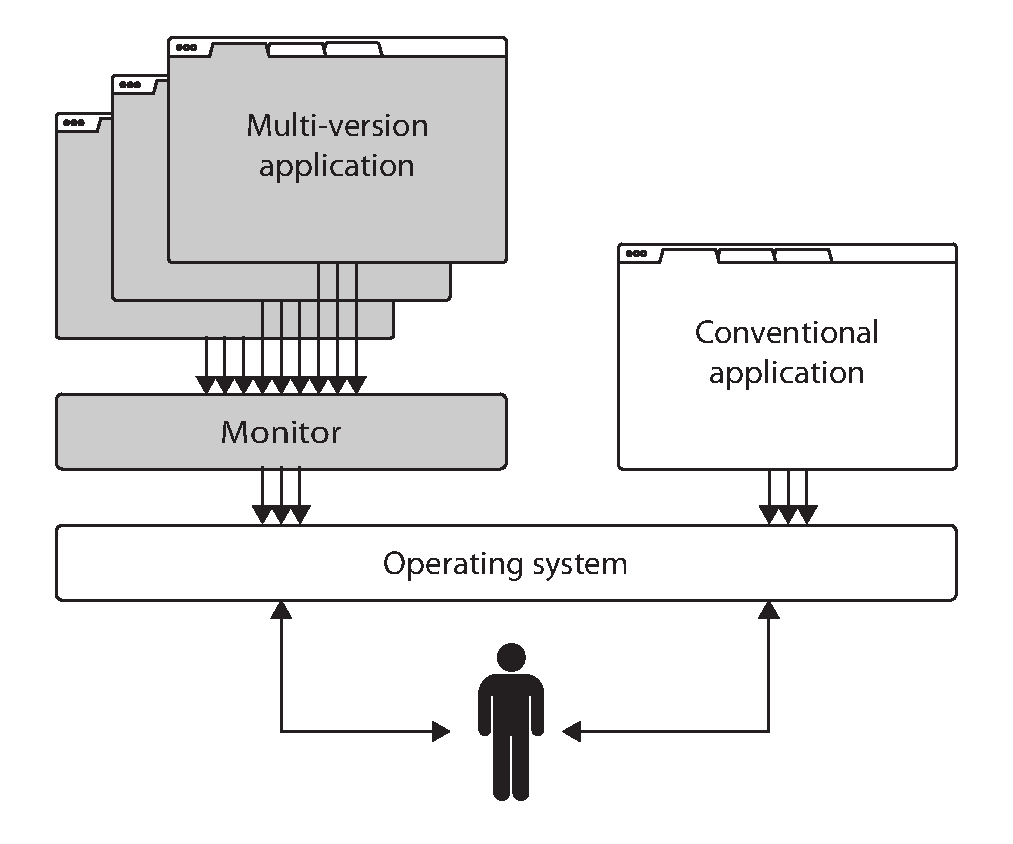
\includegraphics[width=0.5\textwidth]{multi-version/figures/platform}
    \caption{A multi-version execution platform running conventional and multi-version
      applications side by side.}
    \label{fig:mx-platform}
  \end{center}
\end{figure}

To satisfy the first goal, both schemes require a form of virtualization
framework, typically called an \emph{execution monitor}, that would coordinate
the execution of multiple application versions, and mediate their interaction
with the external environment, as shown in Figure~\ref{fig:mx-platform}.
Various such frameworks have been designed in the past in the context of
running multiple automatically generated variants of a given application in
parallel~\cite{diehard06,cox2006,orchestra09}, and some of the techniques
proposed in prior work can be reused in our context. To be practical, this
coordination mechanism has to incur a reasonable overhead on top of native
execution and ensure that the overall system is able to scale up and down the
number of software versions run in parallel in order to balance conflicting
requirements such as performance, reliability, security and energy consumption.

This coordination mechanism can be implemented at multiple levels of
abstraction. The simplest, but least flexible approach is to synchronise the
different versions at the level of application inputs and outputs. This is
particularly suitable for applications that use well-defined protocols such as
web servers and web browsers. The main advantage of this option is that it can
tolerate large differences between different software versions (in fact, one
could even run different implementations, as in \cite{cocktail}), but the main
downside is that it is not applicable in the general case, when the
input-output specification is not available.

A more flexible approach, which we adopted, is to synchronise the different
versions at the level of system calls.  System calls represent the
\emph{external behaviour} of an application, and they are the primary way in
which application interact with the surrounding environment (the other being
shared memory and side channels). While this option allows fewer changes
between different application versions, it does not require any a priori
knowledge of the application's input/output behaviour, and is particularly
suitable in the context of software updates, where the external application
behaviour usually remains unchanged.  In fact, an empirical study presented in
Chapter~\ref{chap:evolution}, which we conducted on several real applications,
has shown that while the source code of these applications changes on a
regular basis, the external behaviour often remains stable when security and
bug fixes are introduced.

% Note that one key aspect on which our approach relies is
% \textit{having the different versions be alive at all times}.  This ensures
% that applications can survive crashes that occur at different points
% in different versions, but adds the extra challenge of restarting
% crashed versions.

%% Once divergences are detected, we need to decide what output should be
%% selected as the output of the multi-version system in order to improve
%% overall reliability.  Many different strategies can be used, but the
%% common goal is to ensure that the multi-version system will have
%% strictly fewer errors than any of the individual versions.

% Finally, our approach needs a deployment strategy to decide what versions are
% run in parallel when the number of available resources (\eg, idle CPU cores) is
% limited.  We envision several options---such as keeping the last $N$ released
% versions (where $N$ is the number of available resources), or keeping several
% very old stable versions---but the exact strategy should be decided on a
% case-by-case basis. % using existing empirical data.

There are several different ways to implement an effective system call monitor,
each with its own set of trade-offs. Solutions targeting binaries are
significantly easier to use, but compared to solutions operating at source code
level, they give up some of the precision while typically requiring more
engineering effort. The most common ways for implementing monitors operating on
binaries are dynamic linking, \ptrace, kernel extensions and binary
instrumentation, while solutions targeting source code typically rely on source
code instrumentation.

System calls are rarely performed directly by the application, which rather use
the wrapper functions provided by the C library. By linking to a custom
library, which provides a custom version of these functions, we could intercept
the system calls performed by the application. This could be done either
statically at link time~\cite{plash}, or dynamically at
runtime~\cite{shepherding:pldi14} (\eg using \lstinline`LD_PRELOAD` or
\lstinline`DYLD_INSERT_LIBRARIES` environment variables). The major benefit of
this approach is efficiency and relative ease of implementation. However, the
mechanism could be easily bypassed (\eg by invoking system calls directly);
also the C library ABI has a significantly larger surface compared to the
system call interface, requiring more engineering effort.

\ptrace is an interface provided by most UNIX-like operating systems, including
Linux, providing the means by which a process might observe and control another
process. The primary use of \ptrace interface is for debugging, but the ease of
use makes \ptrace a popular choice for implementing system call
monitors~\cite{wily-hacker,orchestra09,tachyon12}. \ptrace-based solutions
require relatively low engineering effort, they are easy to deploy and fairly
flexible which makes them especially suitable for rapid
prototyping~\cite{spillane07}.

The use of \ptrace has some drawbacks: a significant performance overhead due
to the large number of context switches, problematic support for multi-threaded
applications, and the lack of a filtering mechanism that would allow
interception only of system calls of interest. \ptrace-based solutions are also
more difficult to debug as the use of \ptrace disallows the use of
\ptrace-based debuggers such as \gdb. The performance overhead could be
partially improved by the use of more efficient mechanism for copying memory
from/to the monitored process, such as shared memory~\cite{orchestra09}, or
cross memory attach (\S\ref{sec:mxm}). The lack of a filtering mechanism could
be addressed by combining \ptrace with the \seccompbpf mechanism~\cite{mbox}.

An alternative to \ptrace is to implement the system call monitor
entirely~\cite{provos2002,cox2006} or partially in kernel space~\cite{ostia}.
While this approach has numerous advantages compared to other approaches, such
as minimal performance overhead and direct access to the application's
execution context and address space, there are several drawbacks.  First, this
approach requires kernel patches and/or new kernel modules which complicates
the development, limits portability across different operating systems or even
different kernel versions, and hinders maintainability. Second, the part of the
monitor that resides in the kernel (\ie kernel module) must be run in
privileged mode, which means that bugs in the implementation may compromise the
system stability. Furthermore, it also makes it difficult for regular users to
deploy and use such monitors.

Binary rewriting techniques allow transforming the executable (either statically
or dynamically) altering its functionality; as such, they can be used to
implement system call monitors by rewriting all system call instructions into 
control flow transfer instructions (\eg
\lstinline[language={[x64]Assembler}]`JMP` instruction). Existing monitors were
built either on top of existing binary rewriting
systems~\cite{onlinevalidation}, or using a purpose-built binary translation
mechanism~\cite{vx32}. The advantage of binary rewriting-based monitors is
relatively low performance overhead, especially in the case of a purposely
built rewriting mechanism. The main disadvantage is the complexity of the
implementation which requires significant development effort.

\subsection{Surviving software errors}

One particular challenge for our approach is to detect any divergences between
different software versions, and resolve them in such a way as to increase the
overall reliability of the application.  Selecting the ``correct'' behaviour of
an application when different versions disagree is not possible in the general
case without having access to a high-level specification.  However, one could%
\begin{inparaenum}[(1)]
\item focus on universal correctness properties, such as the absence of
  crashes, and
\item use various heuristics such as majority voting and favoring the latest
  application versions.
\end{inparaenum}
Our approach is to resolve a divergence by always using the behaviour of the
version that has not crashed, and favour the behaviour of the latest version in
all other cases. %In this way, we ensure that the overall application has fewer
%crashes than any of the individual versions, while still using the new security
%and bug fixes implemented in the latest version.

While this approach is sufficient for the transparent failover scheme, the
failure recovery scheme requires a mechanism for surviving errors in one of the
two versions. Numerous fault recovery techniques have been designed and
described in prior
work~\cite{rx,compl-schedules11,fo,exec-trans06,vigilante,clearview,microreboots,shepherding:pldi14},
but none of these techniques focuses explicitly on faults caused by bugs
introduced by software updates.

We assume that the only difference between the two versions are the changes
introduced by the patch, and that the patch does not modify the internal
application state in a way which would lead to a different behaviour in each
version. We define the internal state of the application as data structures
managed by the application and stored on the stack or heap.

Our solution is based upon the observation that errors in programs are usually
located at particular places (\ie specific instructions) in the program's code.
Therefore, when one of the versions crashes, we can use the code of the other,
non-crashing version to execute over this critical point in that version's
code. This approach may not work when the memory layout of the two versions
differs, as the code of one version may fail to locate the memory structures
necessary for its execution in the memory of the other version.  Nevertheless,
the described approach still works in many cases when the memory layout of the
two versions does not differ significantly
(\S\ref{sec:reliability-evaluation}).

% Given this assumption,  we can recover its internal state from the last
% checkpoint, and then use the code of the other, non-crashing version, to
% execute over the patched region containing the bug, and then recover to the
% original version of the code to continue the execution.
 
\begin{figure}[!t]
  \begin{center}
    \begin{subfigure}[b]{0.45\textwidth}
      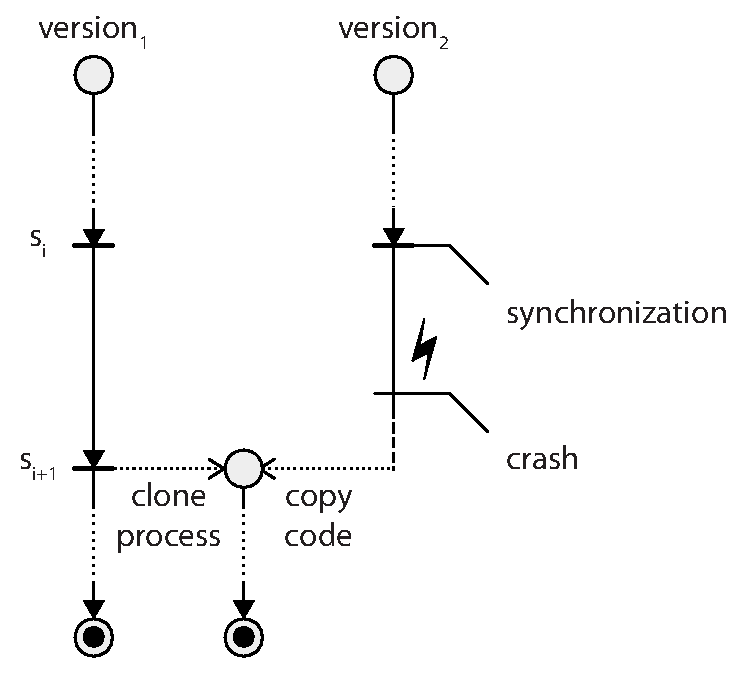
\includegraphics[width=\textwidth]{multi-version/figures/solution1}
      \caption{Patch the text after the crash and continue execution}
      \label{fig:recovery-solution1}
    \end{subfigure}
    \quad
    \begin{subfigure}[b]{0.45\textwidth}
      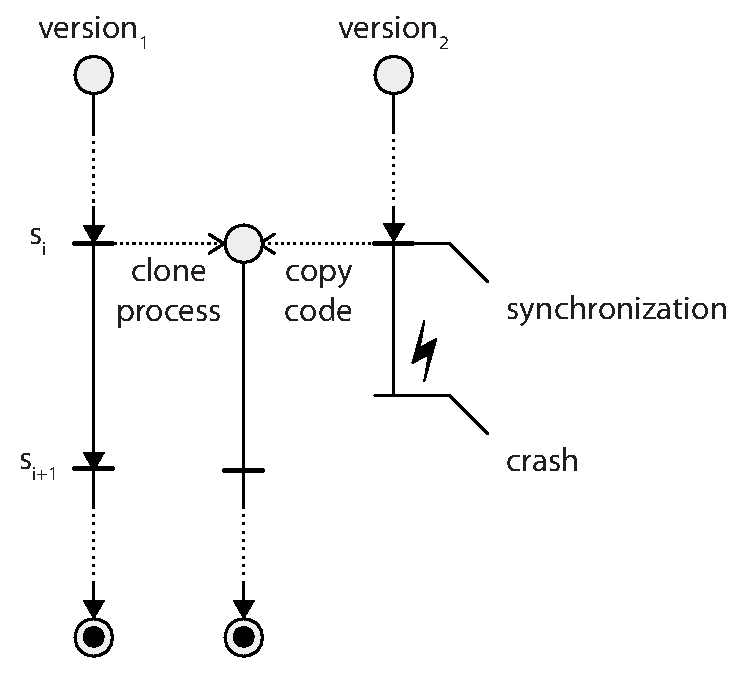
\includegraphics[width=\textwidth]{multi-version/figures/solution2}
      \caption{Patch state before the crash and continue execution}
      \label{fig:recovery-solution2}
    \end{subfigure}
    \quad
    \begin{subfigure}[b]{0.45\textwidth}
      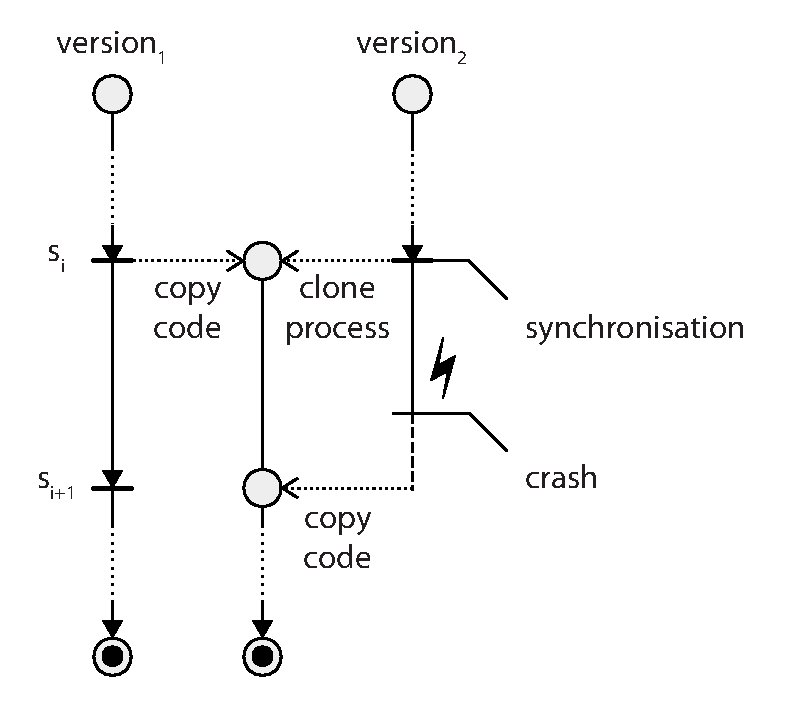
\includegraphics[width=\textwidth]{multi-version/figures/solution3}
      \caption{Use the code of older version only to run through critical section}
      \label{fig:recovery-solution3}
    \end{subfigure}
    \caption{Three solutions for synchronising two divergent versions of the same application}
    \label{fig:recovery-solutions}
  \end{center}
\end{figure}

In our failure recovery approach, we run the two versions in parallel,
monitoring their execution and taking frequent checkpoints at every
synchronisation point, which in our case are system calls. When either of the
versions fails, there are three possible solutions to synchronise the divergent
versions:%
\begin{enumerate}
\item\label{s1} Clone the correctly executing version to duplicate its state
  (\eg memory continents, memory mappings) after the crash and replace its
  code with the code of the failed version. Then restart both versions and
  continue their execution (Figure~\ref{fig:recovery-solution1}).
\item\label{s2} Clone the correctly executing version to duplicate its state at
  the last synchronisation point (\ie creating checkpoint). After the crash,
  replace the code of this cloned version with the code of the failed version.
  Then restart this cloned version, execute over the \emph{critical section},
  and continue execution of both versions
  (Figure~\ref{fig:recovery-solution2}).
\item\label{s3} Clone the failing version to duplicate its state at the last
  synchronisation point. After the crash, replace the code of this cloned
  version with the code of the correctly executing version. Then restart this
  cloned version; after the application successfully executes over the
  \emph{critical section}, replace the code of the cloned version again with
  the original code, and continue its execution
  (Figure~\ref{fig:recovery-solution3}).
\end{enumerate}

While all three solutions can recover the crashing version, in our
implementation we use the third solution as it has the key property of fully
recovering both the code and the state of the crashing version.  This ensures
that applications can survive crashes that occur at different points in
different versions, but adds the extra challenge of restarting crashed
versions. Despite this challenge, we believe this key property is crucial for
the practical application of the multi-version execution technique.

% Our approach aims to provide users with a third choice; when a new version
% arrives, instead of replacing the old version, we run both versions in
% parallel. In our example, consider that we are using \mx to run a
% version of \lighttpd from March 2009.  When the buggy April 2010 version
% is released, \mx runs it in parallel with the old one.  As the two
% versions execute:

% \begin{itemize}
% \item As long as the two versions have the same external behaviour (\eg they
%   write the same values into the same files, or send the same data over the
%   network), they are run side-by-side and \mx ensures that they act as one to
%   the outside world;

% \item When one of the versions crashes (\eg the new version executes the buggy
%   patch), \mx will patch the crashing version at runtime using the behaviour of
%   the non-crashing version.  In this way, \mx can successfully survive crash
%   bugs in both the old and the new version, increasing the reliability and
%   availability of the overall application;

% \item When a non-crashing divergence is detected, \mx will discard one of the
%   versions (by default the old one, but other heuristics can be used).  The
%   other version can be later restarted at a convenient synchronisation point
%   (\eg at the beginning of the dispatch loop of a network server).
% \end{itemize}

% To enable these scenarios, a monitor process coordinates the parallel execution
% of these variants\footnote{The terms \textit{version} and \textit{variant} are
% used interchangeably.} and synchronises their execution, making them appear as
% a single application to any outside entities.  While synchronisation can be
% performed at different levels, the most common approach is to do it at the
% level of system calls, for two main reasons: first, many existing
% diversification transformations, such as address-space layout
% randomisation~\cite{diehard06} and instruction-set
% randomisation~\cite{instr-set-rand03} do not change the sequence of system
% calls (the program's \textit{external behaviour}), and the ordering is often
% preserved even across different software versions.  Second, system
% calls are the main way in which the application communicates with the outside
% environment, and therefore
% %% the ultimate target of attackers.  Finally, as the main
% %% communication mechanism between applications and the environment,
% %% system calls
% must be virtualised in order to enable the multiple versions to act as
% one to the outside world.


